\begin{figure}[h]
    \centering
    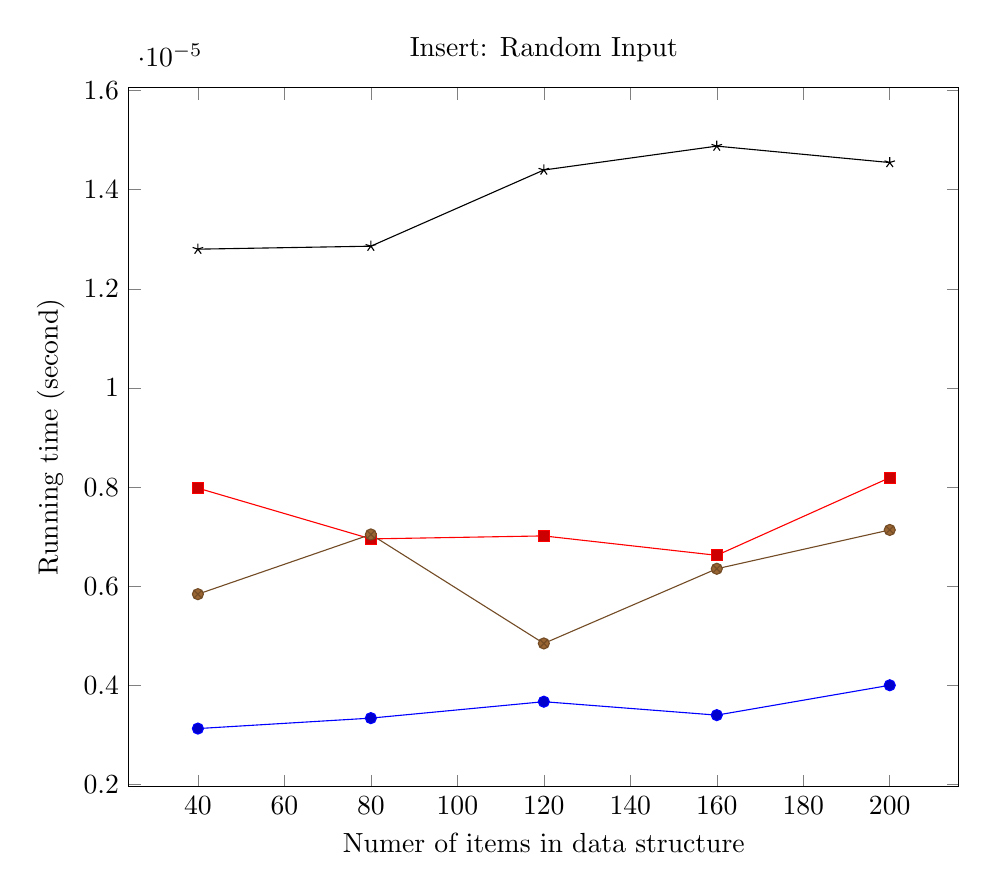
\begin{tikzpicture}
        \begin{axis}[
            xlabel={Numer of items in data structure},
            ylabel={Running time (second)},
            title={Insert: Random Input},
            width=\textwidth
        ]
		\addplot coordinates {
			(40, 3.1322235022175627e-06)
			(80, 3.343046237943431e-06)
			(120, 3.674339108370589e-06)
			(160, 3.403281305294076e-06)
			(200, 4.0056319787974e-06)
		};
		\addplot coordinates {
			(40, 7.98114642391913e-06)
			(80, 6.957150278963722e-06)
			(120, 7.0173853463140205e-06)
			(160, 6.625857408536911e-06)
			(200, 8.191969159645692e-06)
		};
		\addplot coordinates {
			(40, 5.8428015329823476e-06)
			(80, 7.047502879989343e-06)
			(120, 4.848922921701915e-06)
			(160, 6.354799605460399e-06)
			(200, 7.137855481014615e-06)
		};
		\addplot coordinates {
			(40, 1.279995181194607e-05)
			(80, 1.286018687929602e-05)
			(120, 1.439618109673052e-05)
			(160, 1.4878061635532902e-05)
			(200, 1.4546768765105744e-05)
		};
        \legend{}
        \end{axis}
    \end{tikzpicture}
    \caption{Average of 0 operations, benchmarked every 0, starting at 0.}
\end{figure}